\documentclass[12pt,twoside]{mitthesis}

%%%%%%%%%%%%%%%%
%---PACKAGES---%
%%%%%%%%%%%%%%%%
\usepackage{lgrind}
\usepackage{cmap}
\usepackage[T1]{fontenc}
\usepackage{alltt}
\usepackage{fullpage}
\usepackage{multirow}
\usepackage[english]{babel}
\usepackage{color}
\usepackage{colortbl}
\usepackage{natbib}
\usepackage{float}
\usepackage{url}
\usepackage{graphicx}
\usepackage{amsmath}
\usepackage{amsthm}
\usepackage{amssymb}
\usepackage[all]{xy}
% \usepackage{multicol}
% \usepackage{cite}
\usepackage{booktabs}
\usepackage{framed}
\usepackage{dcolumn}
\usepackage[T1]{fontenc}
\usepackage{rotating}
\usepackage{caption}
\usepackage{algorithm}
\usepackage{algpseudocode}




% \pagestyle{plain}


%%%%%%%%%%%%%%%%%%%%%%%%%%%%%%%%%%%%%
%---USER SPECIFIED LaTeX COMMANDS---%
%%%%%%%%%%%%%%%%%%%%%%%%%%%%%%%%%%%%%

\graphicspath{{figures/}}

% Use the bibtex style
\bibpunct{(}{)}{;}{a}{}{,}  % this is a citation format command for natbib
\bibliographystyle{sysbio}

% math options
\DeclareSymbolFont{letters}{OML}{ztmcm}{m}{it}
\DeclareSymbolFontAlphabet{\mathnormal}{letters}

\theoremstyle{plain}
\newtheorem{thm}{\protect\theoremname}
  \theoremstyle{definition}
  \newtheorem{defn}[thm]{\protect\definitionname}
  \theoremstyle{remark}
  \newtheorem{rem}[thm]{\protect\remarkname}

\providecommand{\definitionname}{Definition}
\providecommand{\remarkname}{Remark}
\providecommand{\theoremname}{Theorem}

\floatstyle{plaintop}
\restylefloat{table, sidewaystable}

\definecolor{gray1}{gray}{0.9}
\definecolor{gray2}{gray}{0.5}

\providecommand{\tabularnewline}{\\}
\floatstyle{ruled}
\newfloat{algorithm}{tbp}{loa}
\providecommand{\algorithmname}{Algorithm}
\floatname{algorithm}{\protect\algorithmname}

\newcommand{\comment}[1]{\textbf{[#1]}}


%%%%%%%%%%%%%%%%
%---DOCUMENT---%
%%%%%%%%%%%%%%%%
\begin{document}

\pagenumbering{roman}

% cover I
% blank II
% title page III
% blank IV
% cytat V 
% blank VI
% acknowledgements VII 
% Contents VII 
% blank VIII
% Summary 1 
% blank 2
% Chapter 1 3

%%%%%%%%%%%%%
%---COVER---%
%%%%%%%%%%%%%

%TODO 

%TODO: perhaps move all the proofs to an appendix?

%%%%%%%%%%%%%%%%%%
%---TITLE PAGE---%
%%%%%%%%%%%%%%%%%%
\title{Continous time Markov chain models in phylogenetics and phylogeography; model extension, simulation and visualisation}

\author{Filip Bielejec}

\department{Department of Biomedical Sciences}

\degree{Doctor of Biomedical Sciences}

\supervisor{Philippe Lemey}{Associate Professor}
\supervisor{Guy Baele}{PhD}

\chairman{Chairman}{Chairman}

\degreemonth{November}
\degreeyear{2014}
\thesisdate{\today}

% Make the titlepage based on the above information
\maketitle

%%%%%%%%%%%%%%%%%%%%%%%%
%---ACKNOWLEDGEMENTS---%
%%%%%%%%%%%%%%%%%%%%%%%%
\section*{Acknowledgments}

AAA

% \pagestyle{plain}

%%%%%%%%%%%%%%%
%---CONTENT---%
%%%%%%%%%%%%%%%

\tableofcontents
\pagebreak{}

%%%%%%%%%%%%%%%
%---SUMMARY---%
%%%%%%%%%%%%%%%

\setcounter{page}{1}
\pagenumbering{arabic}

% TODO: unnumbered but mentioned in TOC
\section{Summary}

AAA

%%%%%%%%%%%%%%%%%%%%
%---INTRODUCTION---%
%%%%%%%%%%%%%%%%%%%%
\chapter{Introduction}

\section{General Introduction}

Rapidly evolving pathogens pose an ever increasing threat to the human population.
This threats are exemplified by recent infections with H5N1 avian influenza A, pandemic spread of swine-origin H1N1 influenza \citep{Rambaut2008} or Severe Acute Respiratory Syndrome (SARS) \citep{Ksiazek2003}.
Unlike zoonotic diseases human RNA viruses have no natural barriers that could hamper their escalation.
This is due to the extensive nature of human mobility \citep{Brockmann2006}.

Despite the ever increasing impact of emerging infectious diseases (EIDs) the first studies combining molecular evolution with geographical dispersal are less than 50 years old \citep{Henning1966}. 
Most of these pioneering studies were limited to mapping phylogenetic tip taxa to their geographical coordinates \citep{Kidd2006} and comprehensive quantitative frameworks have only recently begun being developed.

Models that combined the process of spatial diffusion with genetic substitution are only as recent as this decade \citep{Lemey2009,Lemey2010}.
These advances are mostly hampered by the computational burden that they impose.
Finding the maximum likelihood tree requires a search through the space of all possible tree topologies, which quickly becomes computationally intractable, as depicted in Table \ref{tab:maxLikeBurden}.

\begin{table}
\caption{{\bf{Number of rooted trees per number of taxa.}} $4 \times 10^{80} $ is the no of atoms in the observable universe.}
\begin{centering}
\begin{tabular}{cc}
% {@{}l*{2}{D{.}{.}{7}}@{}}
\hline 
Tips & Rooted trees $\frac{(2N-3)!}{2^{N-2}\cdot(N-2)!}$ \tabularnewline
\hline 
\rowcolor{gray1}
$3$ & $3$\tabularnewline
$6$ & $945$\tabularnewline
\rowcolor{gray1}
$9$ & $2'027'025$\tabularnewline
$15$ & $2\times10^{14}$\tabularnewline
\rowcolor{gray1}
$20$ & $8\times10^{21}$\tabularnewline
$55$ & $3.19\times10^{86}$\tabularnewline
\end{tabular}
\par\end{centering}
\label{tab:maxLikeBurden}
\end{table}

Adopting Bayesian statistical approach, implemented in a flexible framework of molecular evolution \citep{Drummond2012} helps circumvent some of these hindrances by focusing sampling efforts on the topologies 
% parts of the tree space
that best fit the data.
Nonetheless Bayesian phylogenetic analyses remain highly computationally intensive and a vast area of research is now aiming at bringing new computational advances to actively stretch these limits \citep{Suchard2009}.

\section{Reconstructing viral spread in time and space}

Central assumption of viral phylogenetics is that thee pidemiological processes that shape the fitness of viral populations leave a measurable footprint on their genomes.
Due to the rapid nature of their evolution this process of character substitution can be observed in almost real time, and gives the opportunity to sample genetic data at different points in time, as opposed to ultrametricly sampled data (\ref{fig:ultrametric}).

%---ULTRAMETRIC TREE---%
\begin{figure}[h]
\begin{center}
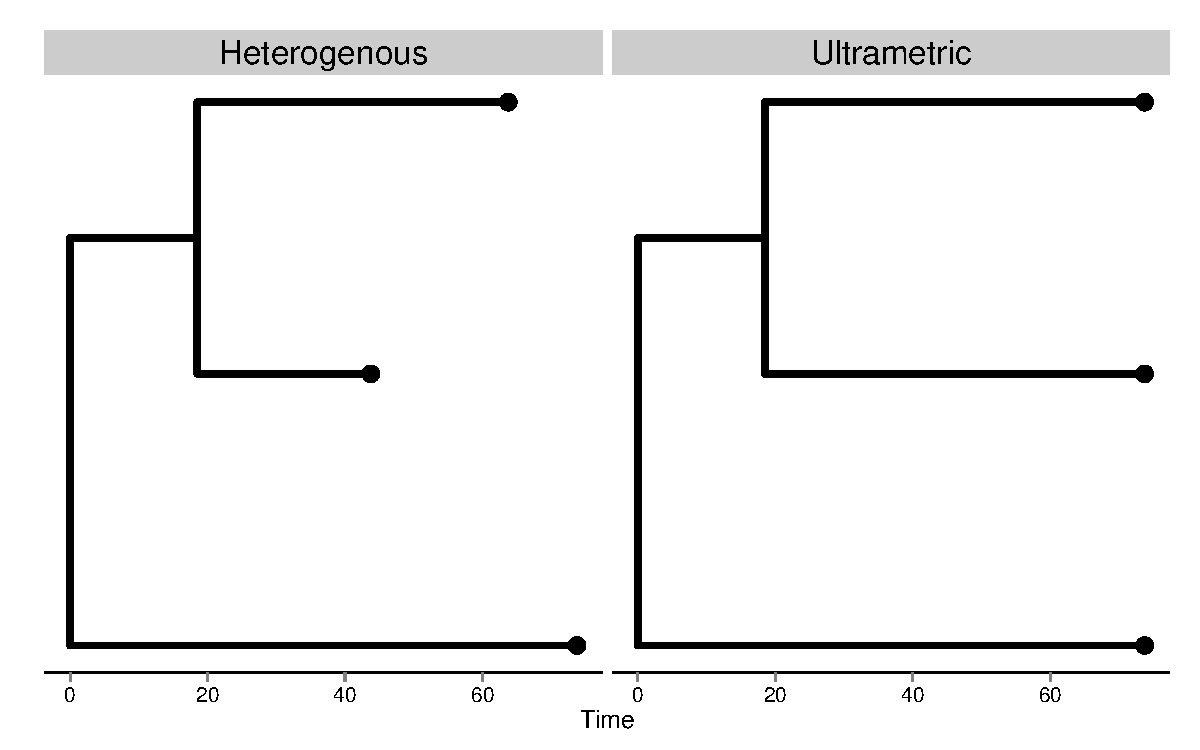
\includegraphics[scale=0.35]{ultrametric} 
\end{center}
\caption{{ \footnotesize {\bf Different sampling schemes.} 
Tree on the right has all of it's sampling dates set at $t=0$. Conversly the tree on the left is sampled at different points in time.
}}
\label{fig:ultrametric}
\end{figure}

Such data-sets are usually reffered to as time-heterogeneous and frequently arise when from studies involving viruses which accumulate statistically significant amounts of genetic change in a relatively short amount of time.
Populations for which such data can be obtained have been called measurably evolving populations (MEPs, cite{Drummond2003}) and have been instrumental in providing  estimates of the evolutionary rate and in advances to the molecular clock models \citep{Drummond2006}.

In studies known as phylodynamics the proceses which shape th eviral genome are integrated with epidemiological dynamics, by assuming that both the evolution and 
geographical dispersal are independent, stochastic processes which unfold on phylogenetic trees.
In that sense the tree is not only a record of evolutionary ancestry, but also of dispersal in actual geographical coordinates, which happen simultaneously.
Our research group has conducts research which aims at developing a full quantitative understanding of the processes that shape the epidemiology and evolution of MEP-like viruses.

% TODO: this is a silly section name; alter
\section{Model extension, simulation and visualisation}

% models
Generally phylogenetic analysis employing stochastic processes make strong restrictive assumptions regarding the underlying substitution process.
They are mainly posited to reduce the number of free parameters of the models describing the molecular evolution and ease both the already mentioned computational tractability and mathematical tractability.
Unfortunately many of these assumptions hamper the application of the methods to real-world, complex data-sets.
Relaxing some of this assumptions and development of more biologically plausibe models, able to grasp the complex nature of phylodynamic dispersal processes is one the aims of the presented thesis \citep{Bielejec2014a}.
Another goal is to make the general applicability suitable for phylogeographic problems as well as beyond them, with potential to turn the findings into usefull predictions of the emergence of infectious diseases, e.g. by identifying the sources and sinks of the geographical dispersal.

% simuation
With the development of novel phylogenetic inference methods comes the need to synthesize evolutionary data in order to compare estimator performance and to characterize strengths and weaknesses of different approaches (e.g. \cite{Arenas2012}, \cite{Hoban2011}).
Whereas the true underlying evolutionary relationships between biological sequences are generally unknown, Monte Carlo simulations allow generating test scenarios while controlling for the evolutionary history as well as the tempo and mode of evolution. 
Part of this thesis is the development and introduction of a flexible utility software for for sequence simulation, that integrates both tree-generative processes as well as models responsible for shaping the molecular histories and geographical dispersal \citep{bielejec2014}.

% visualisation
Phylogenetic inference unevitably results in complex, multi-dimensional output data.
This dimensionality is further incremented by adding the geography to the usuall time-component.
Finally, Bayesian analysis result in posterior distributions of trees, with each tree containing estimated node locations and other traits of interest.
These aspects represent a major challenge for visualizing the inference. 
Yet clear and intuitive visualizations are an important aspect of every analysis (\cite{Hadley10}).
Spatial phylogenetic projections have been undertaken in the field \citep{Kidd06,Parks09}, yet most of these applications remain limited to mapping phylogenetic tip taxa to their geographical coordinates, without providing robust statistical estimates of the geographic locations at the ancestral nodes nor the measures of uncertainty in the inference.
Fortunately the advent of powerful and flexible Geographic Information Systems (GIS) has fostered an interesting possibility in icorporatin both spatial and temporal information into viral phylogenetic analysis.
Presenting readily interpretable visual summaries of the inferences, that can in turn be communicated to the researchers across different fields is one of the more important aspects of this thesis.
This has been materialized in the development of an user-friendly application for producing compelling and informative statistical visualizations of viral spread in time and space \citep{Bielejec2011}.

\chapter{Methodology}

\section{Evolution as a stochastic process}

Molecular phylogenetic modelling typically assumes that the observed molecular sequence data has been generated by some stochastic process, which emits characters over time.
We can think of stochastic processes as functions of time, which is regarded as a deterministic argument, whose values are random (non-deterministic) variables. 
It is thus a statistical model of a random development, or evolution, in time.
Phylogenetic inference often resorts to processes where time is considered to be continuous and the indexed set of outcomes, called the state space, is countable and finite (discrete).
Thus the stochastic process $X$ is a collection $\left\{ X(t)\; t\in T\right\} $, where each drawn value $X(t)$ is a random variable drawn from state space $\mathcal{E}$, with $K$ possible values.

\begin{figure}[H]
\begin{center}
\begingroup
\everymath{\displaystyle}
{\Large
\begin{displaymath} % 
    \xymatrix@R+1pc{ 
\color{gray2}A \ar[r] & \color{gray2}T \ar[r] & A \\
\color{gray2}A \ar[r] & \color{gray2}T \ar[r] & G \\
\color{gray2}A  \ar[rr]_{\tiny \color{gray2}\begin{array}{c}
A\rightarrow G\\
G\rightarrow C
\end{array}} &&  C
% \color{gray1}A \ar[d] & \color{gray1}A\ar[d] & \color{gray1}A\ar[dd]^{\color{gray1}\begin{array}{c}
% A\rightarrow G\\
% G\rightarrow C
% \end{array}}   \\
% \color{gray1}T \ar[d] & \color{gray1}T\ar[d]   \\
% A & G & C 
    } % 
\end{displaymath}
}% END: Large
\endgroup
\end{center}
\caption{{ \footnotesize {\bf Evolution at a single site.} Over time charactes at the site change, leading to the observed data (black). Some of the mutations may be silent. Each site evolves independently.
}}
\label{fig:alignment}
\end{figure}

In the simplest case, for which the unit of evolution is a single nucleotide, we have $\mathcal{E}=\left\{ A,C,G,T\right\}$ and $K=4$.
The particular sites of the alignment are then considered to be stochastically independent realisations of the process $X$, leading to the observed data (see Figure \ref{fig:alignment}). 
As Figure \ref{fig:alignment} depicts not all of the differences can be observed, as due to multiple substitutions (multiple hits) some of the changes are silent.
To accurately describe these processes one needs biologically plausible models of evolution that can grasp their complex nature. 

\subsection{Poisson process}

Poisson process is an example of a continuous-time stochastic process frequently used to describe counts of independent rare events, occuring with some intensity (or rate) $r$, that remains constant over time. 
Among the examples of such process we can mention requests for a single document on a web-server or goals scored in a football game \footnote{Unless it's Real - Barca, than the events are not so rare.}.
The state space in this case is obviously $\mathcal{E} = \left\{ 0,1,2, \dots \right\}$.
This makes Poisson process especially suitable for modelling the timing and number of DNA mutation events. 
Let us formally define a Poisson process.

\begin{defn} 
A Poisson process with rate $r>0$ is continuous-time counting process $\left\{ N(t):\; t\geq0\right\}$ such that:

\begin{itemize}
\item $N(0)=0$.
\item The increments are independent i.e. if $(t_{1},t_{2}]\cap(t_{3},t_{4}]=\emptyset$ then $N(t_2)-N(t_1)$ and $N(t_4)-N(t_3)$ are independent and stationary (i.e. the probability distribution of the number of occurrences counted in any time interval only depends on the length of that interval).
\item The number of events in any interval of length $t$ is $\text{Poisson}(r t)$.
\end{itemize}

Figure \ref{fig:poisson} shows sample trajectories of such a process.

\label{def:poisson}
\end{defn}

% \begin{figure}[H]
% \begin{center}
% 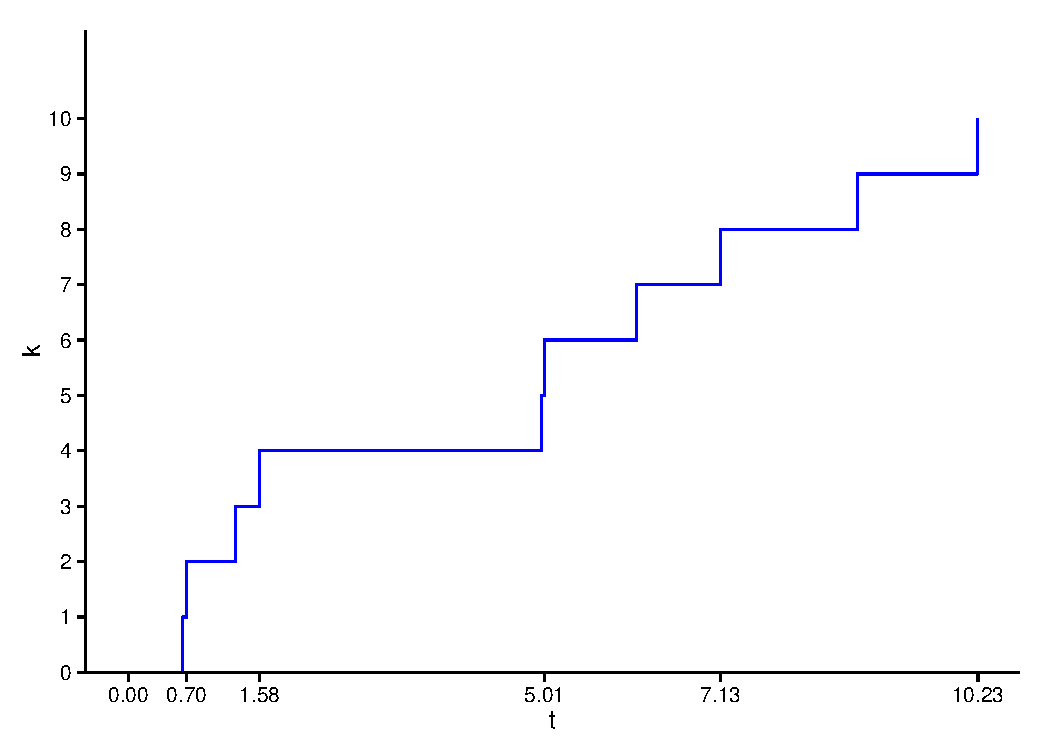
\includegraphics[scale=0.5]{samplepath}
% \end{center}
% \caption{{ \footnotesize {\bf Sample path of the Poisson process with intensity $r=1$.} 
% }}
% \label{fig:poisson}
% \end{figure}
\begin{figure}[H]
\begin{center}
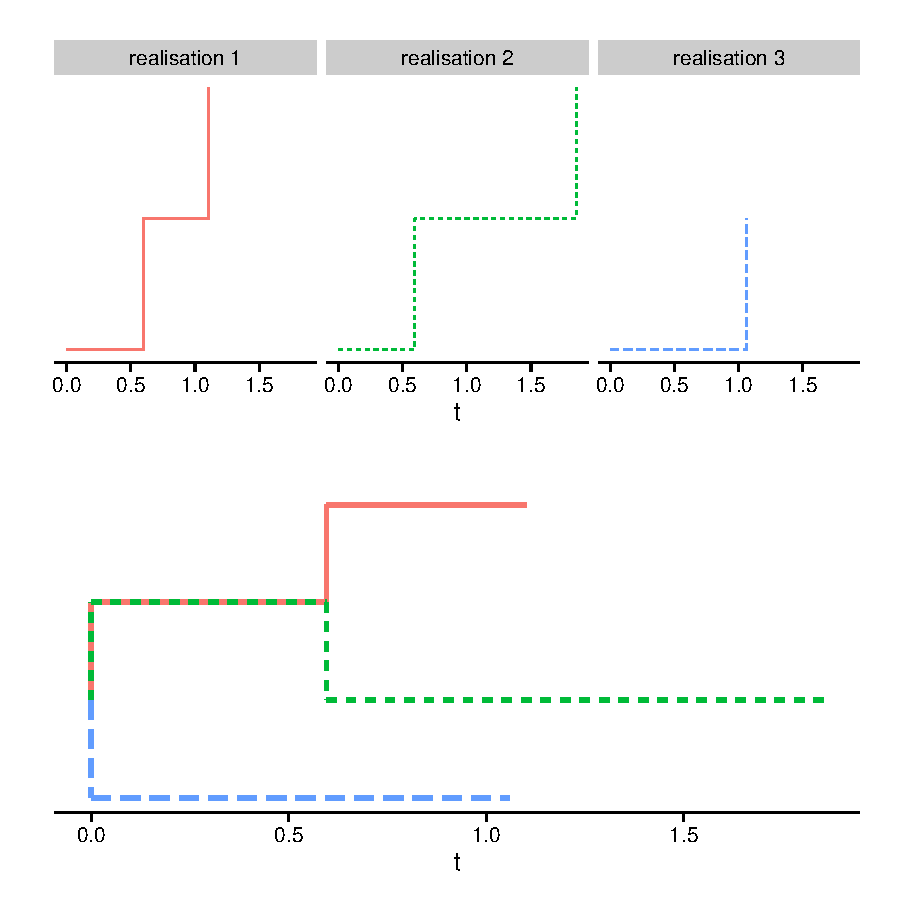
\includegraphics[scale=0.5]{poisson}
\end{center}
\caption{{ \footnotesize {\bf Independent realisations of the Poisson process with intensity $r=1$.}
Times between mutations (the branch lengths) are \emph{iid} exponentially distributed random variables with mean $1/r$.
}}
\label{fig:poisson}
\end{figure}

Let's assume that evolution at a single site is governed by a Poisson process $N$ with some intensity $r$.
From the Definition \ref{def:poisson} under this model the number of mutations $N(t+u)-N(u)$ in some time interval $(u,t+u]$ of length $t$ follows a Poisson distribution with expected number of events $r t$.
Thus we can write:

\begin{equation}
P\left\{ N(t+u)-N(u)=k\right\} =P\left\{ N(t)=k\right\}=\frac{e^{-r t}(r t)^{k}}{k!},\; k=0,1,\ldots
\label{eq:poissonDist} 
\end{equation}

In the Poisson process the time between any two mutations is exponentially distributed with parameter $r$, thus the average waiting time between the arrival of events is $1/r$.
To show this important property we can consider $T_1,T_2,\ldots$ to be the the inter-arrival times, where $T_k$ is the waiting times between the $(k-1)\text{'st}$ and $k\text{'th}$ mutation. 
Obviously the number of mutations before some time $t>0$ is less than some integer $k>0$ if and only if the waiting time $T_k$ until the $k\text{'th}$ mutation is larger than $t$:

\begin{equation}
P\left(N(t)<k\right)=P\left(T_{k}>t\right).
\end{equation}

\noindent
For the first waiting time $T_1$ we have:

\begin{equation}
1-P\left(T_{1}>t\right)=1-P\left(N(t)<1\right)=1-P\left(N(t)=0\right).
\end{equation}

\noindent
From (\ref{eq:poissonDist}) we have that:

\begin{equation}
F_{T_{1}}(t)=1-P\left(T_{1}>t\right)=1-e^{-r t},
\end{equation}

\noindent
therefore $T_1$ follows the exponential distribution with parameter $r$.
For the second waiting time $T_2$ and some arbitrary $u>0$ and $t>0$, by the independent increments property we have that:

\begin{equation}
F_{T_{2}}(t)=1-P\left(T_{2}>t|T_{1}=u\right)=1-P\left(\text{no mutations in }(u,t+u]|T_{1}=u\right)=1-P\left(N(t)=0\right)=1-e^{-r t}.
\end{equation}

\noindent
Therefore $T_2$ is independent of $T_1$ and $\text{Exponential}(r)$. 
Similarly we can show that $T_3$ is indepenent of $T_1$ and $T_2$ and by repeating the same argument $T_1,T_2,\ldots$ are indepenent and identically distributed (i.i.d.) $\text{Exponential}(r)$ random variables.

% TODO: memoryless property does not depend at all, vide poiss)
% TODO: markovian (depends only a little)
% * difference? Memoryless is more

\subsection{Instantaneous rates of mutation}

Within phylogenetic framework one is typically interested not only in modelling the number of events (mutations), but also the actual probabilities of changing states at the particular site in the alignment. 
Let $\mathbf{R}$ denote a $K \times K$ matrix filled with probabilities of exchanging states between any pair $i,j\in \mathcal{E}$.
To express the probability of going from state $i$ to $j$ in some time interval $t$, we multiple the probability of the state change times the probability of having exacly $k$ events leading to the observed change and integrate over all possible values of $k$.
This allows us to accomodate all possible path that the evolution might have taken, and account for multiple hits that might have occured at the site as depicted in Figure \ref{fig:alignment}.
From equation (\ref{eq:poissonDist}) we know the probability of having $k$ mutations in time interval $t$, thus:

\begin{equation}
\left\{ P(t)\right\} _{ij}=\underset{k=0}{\overset{\infty}{\sum}}\mathbf{R}^{k}\frac{(r t)^{k}}{k!}e^{-r t}=\underset{k=0}{\overset{\infty}{\sum}}\frac{(\mathbf{R}r t)^{k}}{k!}e^{-r t},
\end{equation}

\noindent
where $\left\{ P(t)\right\} _{ij}$ denotes the $ij\text{-th}$ element of transition probabilities matrix $\mathbf{P}$ over time $t \geq 0$.
Let us denote the matrix $\mathbf{R}-\mathbf{I}$, where $\mathbf{I}$ is a $K \times K$ identity matrix by $\mathbf{Q}$.
Using the power series definition of the transition probability matrix $exp(\mathbf{R})=\underset{k=0}{\overset{\infty}{\sum}}\mathbf{R}^{k}/k!$ we have:

\begin{equation}
\left\{ P(t)\right\} _{ij}=e^{\mathbf{R}r t}e^{-r t} =e^{(\mathbf{R}-\mathbf{I})r t}=e^{\mathbf{Q}r t} 
\label{eq:matrixExp}
\end{equation}

\noindent
Single entry $q_{ij} \ge 0$ for $i \neq j$ of matrix $\mathbf{Q}$ quantifies the probability of changing from state $i$ to $j$ in an infinitely small amount of time, therefore we will reffer to $\mathbf{Q}$ as the \emph{instantaneous rates matrix}.

\subsection{Computing the matrix exponent \label{sub:exponentiation}}

In order to arrive at the finite-time transition probabilities matrix $\mathbf{P}(t)$ for some time $t\geq0$ one needs to compute the matrix exponential in Equation \ref{eq:matrixExp}.
\cite{Moler78nineteendubious} provide an excellent review of numerical methods to compute the matrix exponent, here we will highlight the method utilized by most phylogenetic software, including BEAGLE \citep{ayres2012beagle} and BEAST \citep{Drummond2012}, that uses the Singular Value Decomposition (SVD) of the rate matrix $\mathbf{Q}$.   

Let us assume $\mathbf{Q}$ has $K$ linearly independent eigenvectors $\mathbf{v}_{i} \; (i=1,\ldots,K)$ with corresponding eigenvalues $\lambda_{i}\;(i=1,\ldots,K)$:

\begin{equation}
\mathbf{Q}\times\mathbf{V}=\lambda\times\mathbf{V}
\label{eq:eigenvaluesEigenvectors}
\end{equation}

\noindent
This condition is sufficient for $\mathbf{Q}$ to be diagonizable, thus it's Jordan form is:

% TODO: format
\begin{equation}
\mathbf{V}\times\mathbf{Q}\times\mathbf{V}^{-1}=\left[\begin{array}{cccc}
\lambda_{1} & 0 & \cdots & 0\\
0 & \lambda_{2} & \ddots & \vdots\\
\vdots & \ddots & \ddots & 0\\
0 & \cdots & 0 & \lambda_{K}
\end{array}\right]=\text{diag}(\lambda_{1},\ldots,\lambda_{K})=\mathbf{D} ,
\label{eq:diagonalization}
\end{equation}

\noindent where $\mathbf{V}$ is a matrix composed of eigenvectors of $\mathbf{Q}$. 
Multiplying both sides of equation (\ref{eq:diagonalization}) with the edge length $t$ and scaled by the appropriate rate scalar $r$, we can write $\mathbf{Q}$ in form:

\begin{equation}
rt\mathbf{Q}=\mathbf{V}\times\text{diag}(rt\lambda_{1},\ldots,rt\lambda_{K})\times\mathbf{V}^{-1} .
\end{equation}

\noindent Finally, using the power series definition of the transition probability matrix: 

\begin{eqnarray}
\mathbf{P}(t) & = & \exp\left(rt\mathbf{Q}\right) \\ \nonumber
& = & \underset{k=0}{\overset{\infty}{\sum}}\left(rt\mathbf{Q}\right)^{k}/k! \\ \nonumber
& = & \underset{k=0}{\overset{\infty}{\sum}}\left(\mathbf{V}\times\mathbf{D}\times\mathbf{V}^{-1}\right)^{k}/k! \\ \nonumber
& = & \mathbf{V}\times\left(\underset{k=0}{\overset{\infty}{\sum}}\mathbf{D}^{k}/k!\right)\times\mathbf{V}^{-1} \\ \nonumber
& = & \mathbf{V}\times\text{diag}(e^{rt\lambda_{1}},\ldots,e^{rt\lambda_{K}})\times\mathbf{V}^{-1} ,
\label{eq:eigen_decomposition}
\end{eqnarray}

\noindent 
where the last transition is due to the fact that exponential of diagonal matrix is obtained by exponentiating every entry on the main diagonal.
We should note here that the tepeated evaluations of $\exp\left(rt\mathbf{Q}\right)$ for different times $t$ are all based on the same SVD of the matrix $\mathbf{Q}$. 
One needs only to scale and exponentiate the eigenvalues to calculate the diagonal matrix $D$ and perform two matrix multiplications, thus reducing all calculations to a simple and effective algorithm. 

\subsection{Markov chain models of sequence substitution}
% TODO markov property is inherited from Poisson process
Drawing realizations with probabilities defined by $\mathbf{P}$  gives rise to a continuous-time stochastic process $\left\{ X(t):\; t\geq0\right\}$ satisfying the Markov property, such that for every $n\geq 0$, given the time points $0\leq t_{0}\leq t_{1}<\ldots<t_{n}\leq t_{n+1}$ and discrete states $i_{0},i_{1}, \ldots, i_{n},i_{n+1}$ it holds that: 

\begin{eqnarray}
P\left\{ X(t_{n+1})=i_{n+1}\mid X(t_{n})=i_{n},\ldots, X(t_{0})=i_{0}\right\} =P\left\{ X(t_{n+1})=i_{n+1}\mid X(t_{n})=i_{n}\right\} .
\label{eq:markov}
\end{eqnarray}

The elements of $\mathbf{P}$ quantify the finite-time transition probabilities between the $K$ discrete state-space elements.
We have described here a Continuous-time Markov chain (CTMC), that we will use to describe the substitution process at a single site of an alignment.
% TODO: completely characterized by Q
Every CTMC is completely characterized by its rate matrix $\mathbf{Q}$ and the stochastic matrix $\mathbf{P}(t),\ t\geq0$ is obtained via matrix exponentiation as decibed in Subsection \ref{seq:exponentiation}.

%---SUBSTITUTION MODEL---%
\begin{figure}[h]
\begin{center}
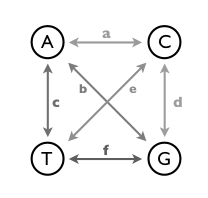
\includegraphics[scale=0.5]{substitution} 
\end{center}
\caption{{ \footnotesize {\bf  Nucleotide substitution model.} 
% Markov substitution models provide the cornerstone of computational phylogenetics.
}}
\label{fig:substitution}
\end{figure}

Figure \ref{fig:substitution} depicts an example of such a CTMC substitution model, describing the process of substitution between four discrete nucleotide base pairs, where all the pairs communicate (all states have a non-zero transitional probability of exiting from, i.e. all states are non-absorbing).
Let us denote a transition probability between two states $i$ and $j$ over time $u$ to $t+u$ by:

\begin{equation}
p_{ij}\left(u,t+u\right)=P\left\{ X(t+u)=j\mid X(u)=i\right\} .
\end{equation}

In the phylogenetic setting, researchers often constrain the CTMC processes, mostly for computational and mathematical convenience.
One of the restrictions is the assumption of time-homogeneity of the substitution process, which states that the evolution does not change in pattern over time and therefore transition probabilities depend only on the difference $t$ between times $u$ and $t + u$:

\begin{equation}
p_{ij}\left(t\right) = p_{ij}\left(0,t\right) = p_{ij}\left(u,t+u\right).
\label{eq:time_homogeneity}
\end{equation}

Unfortunately this assumption clearly does not hold for many real-world data-sets, as the temporal dynamics clearly do shift in time, often in a seasonal, observable manner \citep{Bahl2011}.
One of the goals of the research presented in this thesis is the development of a model that can grasp such situations.

Substitution models are further constructed to be ergodic, meaning that there exist positive values $\pi_{1},\pi_{2},\ldots,\pi_{K}$ such that:

\begin{equation}
\forall i,j\in \mathcal{E}  \quad\underset{t\rightarrow\infty}{lim}p_{ij}(t)=\pi_{j}.
\label{eq:ergodicity}
\end{equation}

As $t$ goes to infinity the probability that the site is in some state $j$ is non-zero and does not depend on the starting state $i$.
This implies that the chain will always display the same long-term behavior, which is why $\mathbf{\Pi}=\{\pi_{i},\ i\in\mathcal{E}\}$ is called a \emph{stationary distribution} (also referred to as the \emph{equilibrium distribution} or \emph{equilibrium frequencies}).
We can look at the elements of $\mathbf{\Pi}$ as the proportion of time spent in states $i\in\mathcal{E}$ after the Markov chain has run for infinitely long time, that does not depend upon the initial state of the process.
In other words if we sample the initial state from the stationary distribution and then let the process run for some sufficiently long time $t$, then the distribution of the final state will equal the stationary distribution. 

Another commonly applied constraint is that of \emph{time-reversibility}, meaning that the model does not care which character is the ancestor and which is the descendant so long as all other parameters are held constant.
For all $i,j\in \mathcal{E}$ and $t\geq 0$ we have:

\begin{equation}
\pi_{i}p_{ij}(t)=\pi_{j}p_{ji}(t).
\label{eq:time_reversibility1}
\end{equation}

\noindent
Condition \ref{eq:time_reversibility1} is also referred to as the \emph{detailed balance} equation, and posits that the probability of sampling $i$ from the stationary distribution and then going to $j$ over some finite-time $t$ is the same as sampling $j$ and going to $i$. 
% By the definition of $\mathbf{\Pi}$ and $\mathbf{P}$ from (\ref{eq:time_reversibility1}) we have:
% 
% \begin{equation}
% \pi_{i}q_{ij}=\pi_{j}q_{ji}\mathbf{Q}.
% \label{eq:time_reversibility2}
% \end{equation}
% 
% Definition (\ref{eq:time_reversibility1}) and (\ref{eq:time_reversibility2}) are equivalent.
This condition is assumed for strictly computational reasons, i.e. time-reversibility makes it easier to diagonalize $\mathbf{Q}$, which as we have described in 
Subsection \ref{seq:exponentiation} is a strategy frequently employed in phylogenetic software to compute the exponentials of rate matrices.
Time reversibility also simplifies the computation of the likelihood on a tree, since it is then indifferent to the position of the root, which we will discuss in Subsection \ref{seq:likelihood}.

%TODO: GTR as example? see M USYB 4

\subsection{Phylogenetic tree}

A phylogenetic tree, or phylogeny for short, depicts the genealogical relationship between character sequences.
Mathematically, a phylogeny $\mathbf{F}$ represents a directed, acyclic graph with sets of \emph{nodes} connected by \emph{branches} (e.g., Figure \ref{fig:treeconcept}).
Data is observed only at the external nodes (\emph{tips}), while internal nodes represent extinct ancestors for which data is usually missing.
The ancestor of all observed samples is called the \emph{root} of the tree and it's height is reffered to as the time to the most recent common ancestor (TMRCA).

%---TREE CONCEPT---%
\begin{figure}[H]
\begin{center}
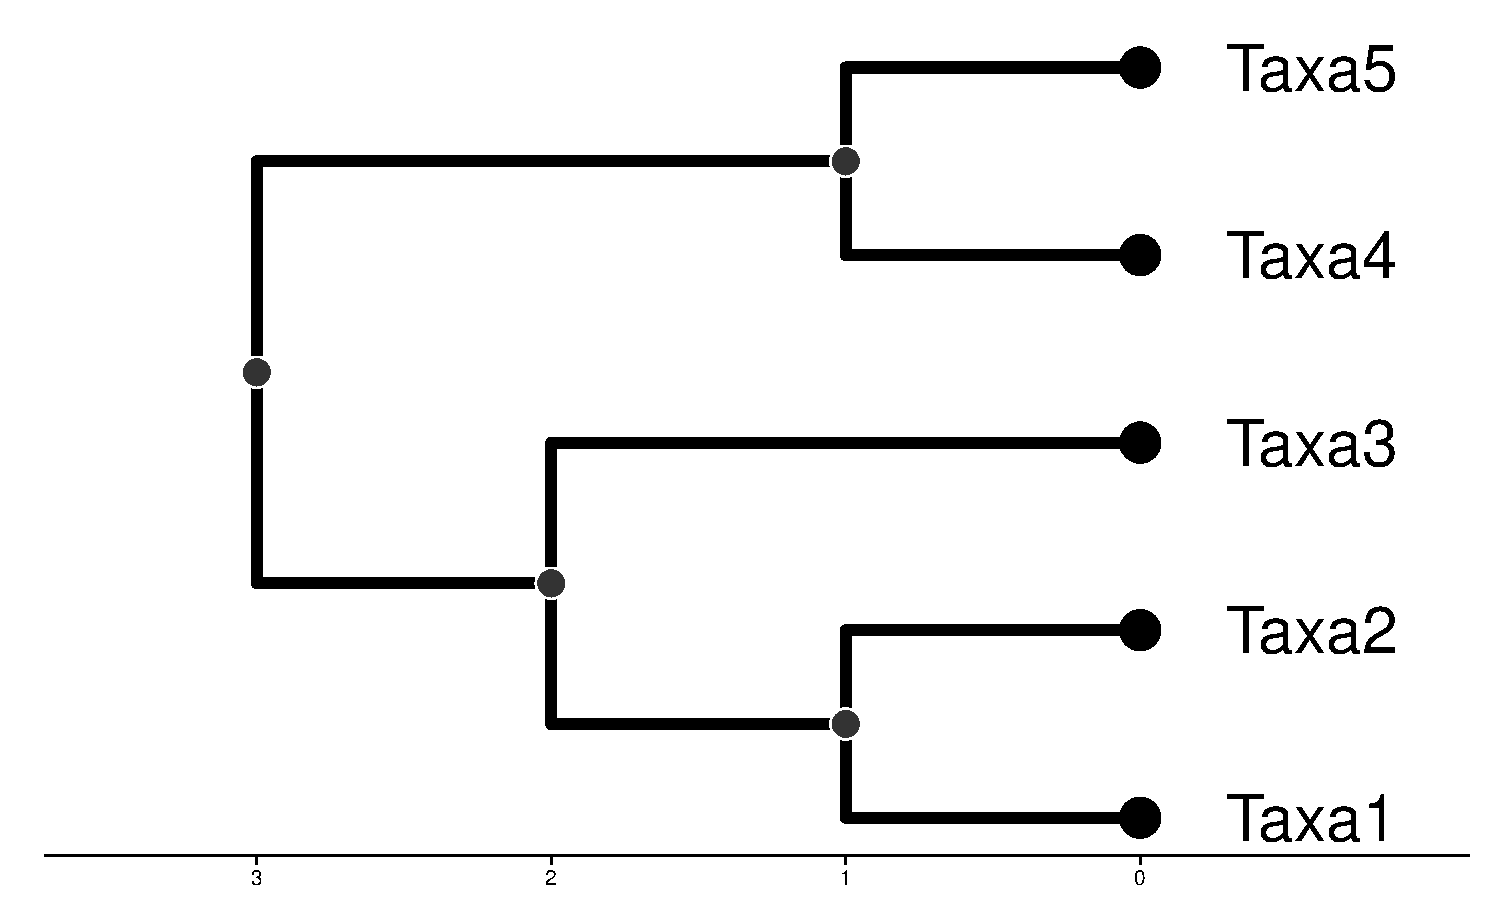
\includegraphics[scale=0.35]{treeconcept} 
\end{center}
\caption{{ \footnotesize {\bf A phylogenetic tree showing evolutionary relationships.} 
Character sequences are observed at the tips of the tree (black dots); sequence characters at the internal nodes are treated as missing data. 
Branch lengths are estimated in units of genetic distance, or in this case, real time.
}}
\label{fig:treeconcept}
\end{figure}

Within our framework we focus on trees which are rooted and time-measured, i.e. their branch lengths are scaled in actual time units.
A rooted binary tree with $n$ leaves has $2n-2$ branches and $n-1$ internal nodes.
The branching pattern of the tree is called the \emph{topology}. 

\subsection{Sequence evolution on a tree\label{sub:evolutionOnTree}}

We now move onto describing the connection between already discussed CTMC models of character sequence evolution and the phylogenetic trees.
Like before we focus on a single site of the alignment, and due to the assumption of independence the probability of an alignment is simply the product of probabilities calculated at individual sites.

To gain a better understanding of the process shaping the data observed at the tips of a phylogenetic tree let us consider the probelm of simulating a sequence evolution on a tree.
We start with a first character $i$ sampled at the root of the tree $x_0$ from the stationary distribution $\mathbf{\Pi}$.
Let us assume that two directly neighboring nodes are $x_j$ and $x_k$.
The character sampled at the root waits an Exponentialy distributed amount of time $t\geq0$ (see Figure \ref{fig:poisson}) before moving down the tree to one of the children nodes $x_i$.
Such traversal is said to be following the pre-order, i.e. parental nodes are visited before child nodes.   
The process then randomly decides by a coin flip to which of the two neighbouring nodes to move next.
Let us assume that the process moved to $x_j$.
The state $j$ for the node $x_j$ is sampled conditional on the value $i$ already sampled at the root using the branch length expressed in real time $t$ and the vector probabilities in the row $i$ of the finite-time probabilities matrix $\mathbf{P}(t)$, calculated using SVD of the rate matrix $\mathbf{Q}$ that characterizes the CTMC.   

\begin{algorithm}
\begin{center}
\begin{algorithmic}[1]
\footnotesize{
%
\State $node \gets getRoot\left(\right)$
%
\State $state \gets getState\left(node\right)$
%
\Repeat
%
\If{$\left(hasChildren\left(node\right)\right)$}
%
\ForAll{children}
%
\State $t \gets getDistanceToParent\left(child\right);$
%
\State $ \mathbf{P}\left(t\right) \gets e^{\mathbf{Q}t};$
%
\State $state \gets sample\left(\mathbf{P}\left[ state, \right]\right);$
%
\EndFor
%
\Else \Comment{this is tip node}
%
\State $node \gets getParent\left(node\right);$
%
\EndIf
%
\Until{$\left(\text{simulated for all nodes}\right)$}
}
\end{algorithmic}
\end{center}
\caption{{ \footnotesize {\bf Fabrication evolution along a phylogeny.} 
For a visited child node it's state is sampled with conditional probabilities of changing to state $j$ given state $i$ at the parental node.
}}
\end{algorithm}

This constitutes the Markov property of a CTMC, as defined in (\ref{eq:markov}).
The sampling is then repeated on the node $x_j$, before recursively proceeding to the other trio of nodes.
The states sampled at the tips of the tree constitute the character sequence for one site of the alignment.
In thi slight the CTMC process can be viewed as a continuous-time random-walk, unfolding on the topology $\mathbf{F}$, with it's behaviour described by a rate-matrix $\mathbf{Q}$.

\section{Likelihood of sequence evolution}

\subsection{Calculation of the Likelihood on a tree\label{seq:likelihood}}

Likelihood is defined as a conditional probability of observing the data given the parameters, in a function of those parameters.
Discrete molecular sequence data comes in a form of aligned matrix $\mathbf{X}$ of size $n \times l$, where $x_{jh}$ is the $h$-th character in $j$-th sequence.
Single column $\mathbf{x}_{h}$ of data matrix constitutes a single site.
Like before the standard assumption of independence posits that different sites evolve independently and that once two branches split at a node the evolution on those is also independent.

In Subsection \ref{sub:evolutionOnTree} we described how some process $\mathbf{Q}$ gives rise to the observed data $\mathbf{X}$.
In the typicall situation we start with just the observed data and aim the inference efforts at modelling the process that generated the alignment.
We can therefore denote the likelihood simply as: 

\begin{equation}
L\left(\mathbf{\theta}|\mathbf{X}\right)=P\left(\mathbf{\theta}|\mathbf{X}\right), 
\label{eq:likelihood}
\end{equation}

\noindent
where $\theta$ it the topology, branch lengths, parameters of the substitution model and other parameters of interest that we aim at estimating.
This quantity expresses how likely it is to observe the data given a specific value of the parameter of interest $\theta$.
By finding the value of $\theta$ that maximizes (\ref{eq:likelihood}) we capture a model with the best possible fit.

In this thesis we will not discuss the maximum likelihood estimation itself, rather focus on closely related methods of Bayesian inference.
The likelihood is nontheless required for both methods of inference, hence we will now discuss how to calculate the likelihood of observing a certain realised sequence of characters on a tree, given a substitution model.

%---LIKELIHOOD---%
\begin{figure}[h]
\begin{center}
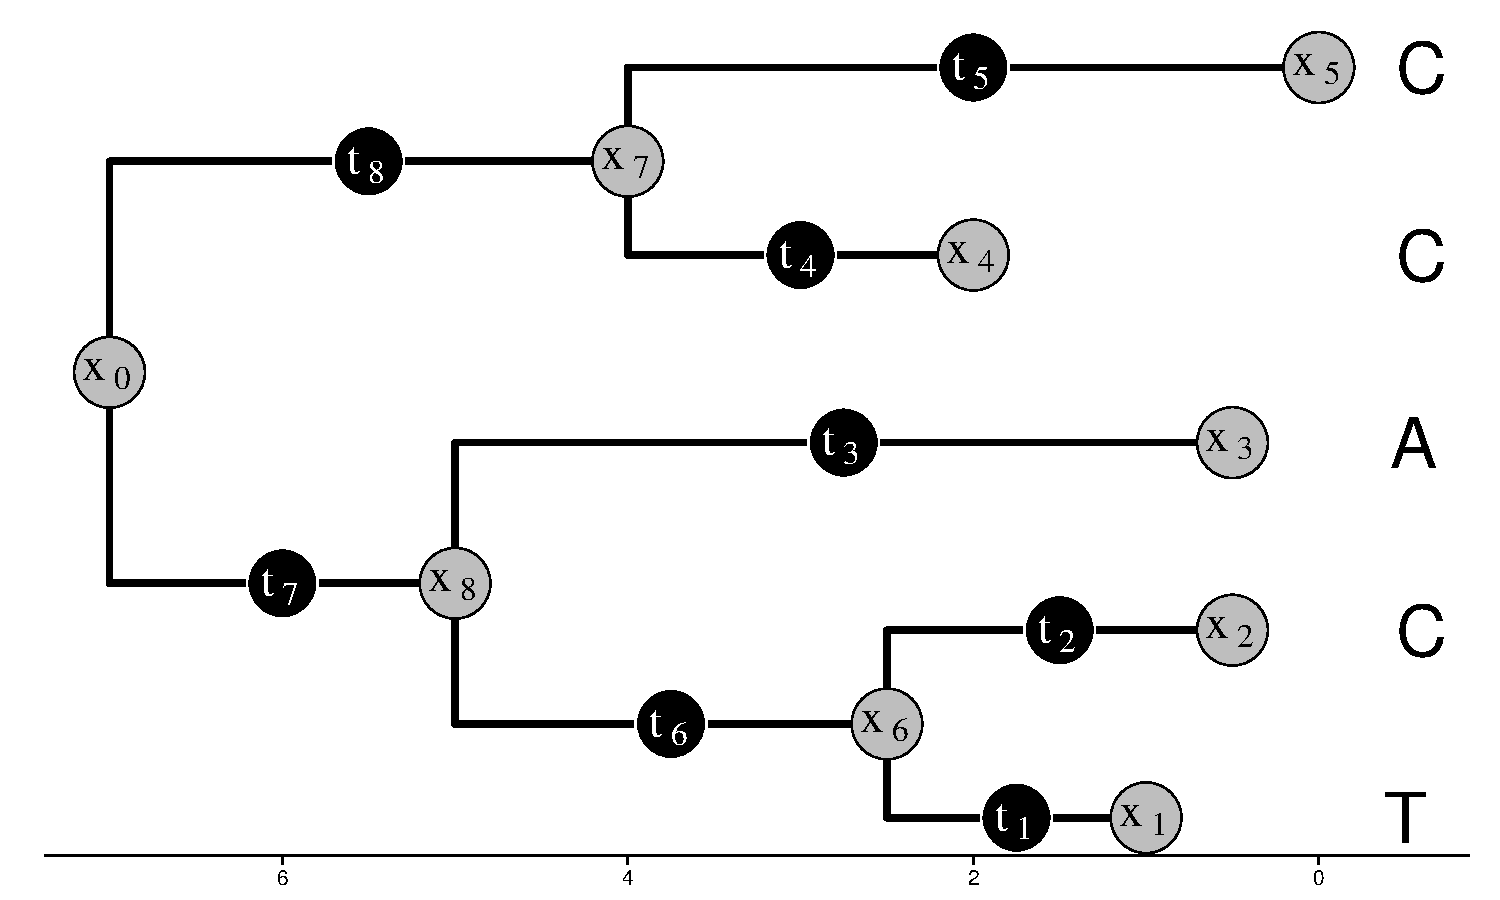
\includegraphics[scale=0.5]{likelihood} 
\end{center}
\caption{{ \footnotesize {\bf  A tree with five taxa.} 
Character sequence data for single site is observed at the tips of the tree.
}}
\label{fig:LIKELIHOOD}
\end{figure}

To calculate the likelihood means thus to reverse-engineer the evolution as it happened.
Figure \ref{fig:LIKELIHOOD} presents single site $TCACC$ observed at the tips of the tree.
External nodes are numbered $x_{1}, \ldots x_{5}$, internal nodes $x_{6}, \ldots x_{8}$ and the root is placed at the node $x_{0}$.
Length of each branches leading to node $i$ is denoted as $t_{i}$.
Using methods presented in Subsection \ref{sub:exponentiation} we calculate the finite-time transition probabilities $p_{ij}(t_{i})$ between all pairs of characters in the alignment.
According to the independence assumptions to calculate the probability at a single site we need to sum over all possible combinations that could give rise to the observed sequence. Thus:

\begin{equation}
\underset{X_{0}\in S}{\sum}\underset{X_{6}\in S}{\sum}\underset{X_{7}\in S}{\sum}\underset{X_{8}\in S}{\sum}[\pi_{x_{0}}\cdot p_{x_{0}x_{8}}(t_{7})\cdot p_{x_{0}x_{7}}(t_{8})\cdot p_{x_{8}x_{6}}(t_{6})\cdot p_{x_{8}A}(t_{3})\cdot p_{x_{7}C}(t_{4})\cdot p_{x_{7}C}(t_{5})\cdot p_{x_{6}T}(t_{1})\cdot p_{x_{6}C}(t_{2})]
\label{eq:likelihood}
\end{equation}

We can break down the terms in (\ref{eq:likelihood}) to the probability of observing the data $TCACC$ for the tips and $x_{0},x_{6},x_{7},x_{8}$ for the ancestral nodes (inside the brackets) and the sum over all possible combination over the state space $S$ (outside the brackets).
Term $\pi_{0}$ is simply the probability that the root has character $x_{0}$ and comes from the assumption that the process generating the data has reached its equilibrium.

Summing over all possible paths leading to the observed data is computationally expensive, as there are  $K^{n-1}$ possible combinations, where $n-1$ is the number of internal nodes of a rooted binary tree.
Fortunately we can used the assumption of independence of the process in the two sub-trees below every node.
\citet{Felsenstein1981} provides an efficient algorithm for computing the likelihood of observing the data on a topology $\mathbf{F}$ given the substitution model that quantifies transition probabilities.
This routine, known as \emph{tree pruning} conveniently expresses the partial likelihood $L_{i}(x_{i})$ of observing data at the descendant tips of node $i$ given state $x_{i}$ at node $i$ in terms of partial likelihoods at nodes $j$ and $k$.
For all internal nodes of $\mathbf{F}$ we have:

\begin{equation}
L_{i}(x_{i})=\left[\underset{x_{j}\in \mathcal{E}}{\sum}\mathbf{P}_{x_{i}x_{j}}(t_{j})L_{j}(x_{j})\right]\times\left[\underset{x_{k}\in \mathcal{E}}{\sum}\mathbf{P}_{x_{i}x_{k}}(t_{k})L_{k}(x_{k})\right]
\label{eq:felsenstein1}
\end{equation}

\noindent
For tip nodes we have:

\begin{equation}
L_{i}(x_{i})=\begin{cases}
1 & \text{if }\hat{x}(i)=x_{i}\\
0 & \text{otherwise}
\end{cases},
\label{eq:felsenstein2}
\end{equation}

\noindent
where $\hat{x}(i)$ denotes the character state observed at node $i$.
After recursively applying (\ref{eq:felsenstein1}) to all the nodes of $\mathbf{F}$ in post-order fashion the likelihood of the data at the site is given by:
% we can integrate out the unobserved states calculating successive contributions to the partial likelihood.

\begin{equation}
L(\mathbf{x}_{h})=\underset{x_{0}\in\mathcal{E}}{\sum}\pi_{x_{0}}\cdot L_{0}(x_{0})
\label{eq:felsenstein3}
\end{equation}

\noindent
The log-likelihood of the whole alignment $X$ is computed by summing the logarithms of the likelihoods at the particular sites, due to the assumption of their independence:

\begin{equation}
l(X)=\underset{j=1}{\overset{l}{\sum}}log\left(L(\mathbf{x}_{jh})\right)
\label{eq:loglikelihood}
\end{equation}

\subsection{Computational burden}

% define o notation

Calculating the log-likelihood of the tree involves:

\begin{enumerate}
\item { Singular value decomposition of the rate matrix $\mathbf{Q}$. }
\item { Taking the exponential of $\mathbf{Q}t$ for each branch length $t$. }
\item { Applying (\ref{eq:felsenstein1}) for every site in the alignment and every possible state in the state space $\mathcal{E}$. }
\item { Taking the logarithm and summing over all sites in the alignment. }
\end{enumerate}

Step (1) proceeds at ${\cal{O}}(K^3)$, however for typical, time-homogeneous applications this is not the a rate-limiting step, as repeated evaluations of $exp(\mathbf{Q}t)$ in (2) are based on the same decomposition of the matrix \citep{Suchard2009}. 
Step (2) typically boils down to repeated matrix-vector-matrix multiplications and its serial computational order is ${\cal{O}}(K^3 \times n)$. 
Step (3) takes ${\cal{O}}(K^2 \times n \times l)$ time and is the most computationally expensive part of the routine. 
Step (4) proceeds at ${\cal{O}}(l)$, linearly with the number of sites.
Fortunately these operations are very regular and lend themselves to the computational parallelism, such as utilized in the BEAGLE library \citep{Suchard2009,Ayres2012}.

% I skipped site rate variability, but perhaps it should be mentioned? 
























%%%
\section{Bayesian inference}

\subsection{Bayes theorem}

\subsection{Marcov Chain Monte Carlo}

%%%
\section{Bayesian phylogeography}

%%%%%%%%%%%%%%%%%
%---CHAPTER 1---%
%%%%%%%%%%%%%%%%%
\chapter{Modelling substitution heterogeneity through time}


%%%%%%%%%%%%%%%%%
%---CHAPTER 2---%
%%%%%%%%%%%%%%%%%
\chapter{Visualizing viral spread in time and space}


%%%%%%%%%%%%%%%%%
%---CHAPTER 3---%
%%%%%%%%%%%%%%%%%
\chapter{Evolutionary simulation}


%%%%%%%%%%%%%%%%%
%---CHAPTER 4---%
%%%%%%%%%%%%%%%%%
\chapter{Branch specific codon models}


%%%%%%%%%%%%%%%%%%%%
%---BIBLIOGRAPHY---%
%%%%%%%%%%%%%%%%%%%%
\bibliography{thesisrefs}

\end{document}

